
% \tm{I've removed the 'Examples' section header and just put these into 'example' environments. We are going to need the space later :)}

\begin{comment}
\begin{example}[Example~\ref{example:coin} with Plan~\ref{plan1}]
% \begin{figure}
%     \centering
%     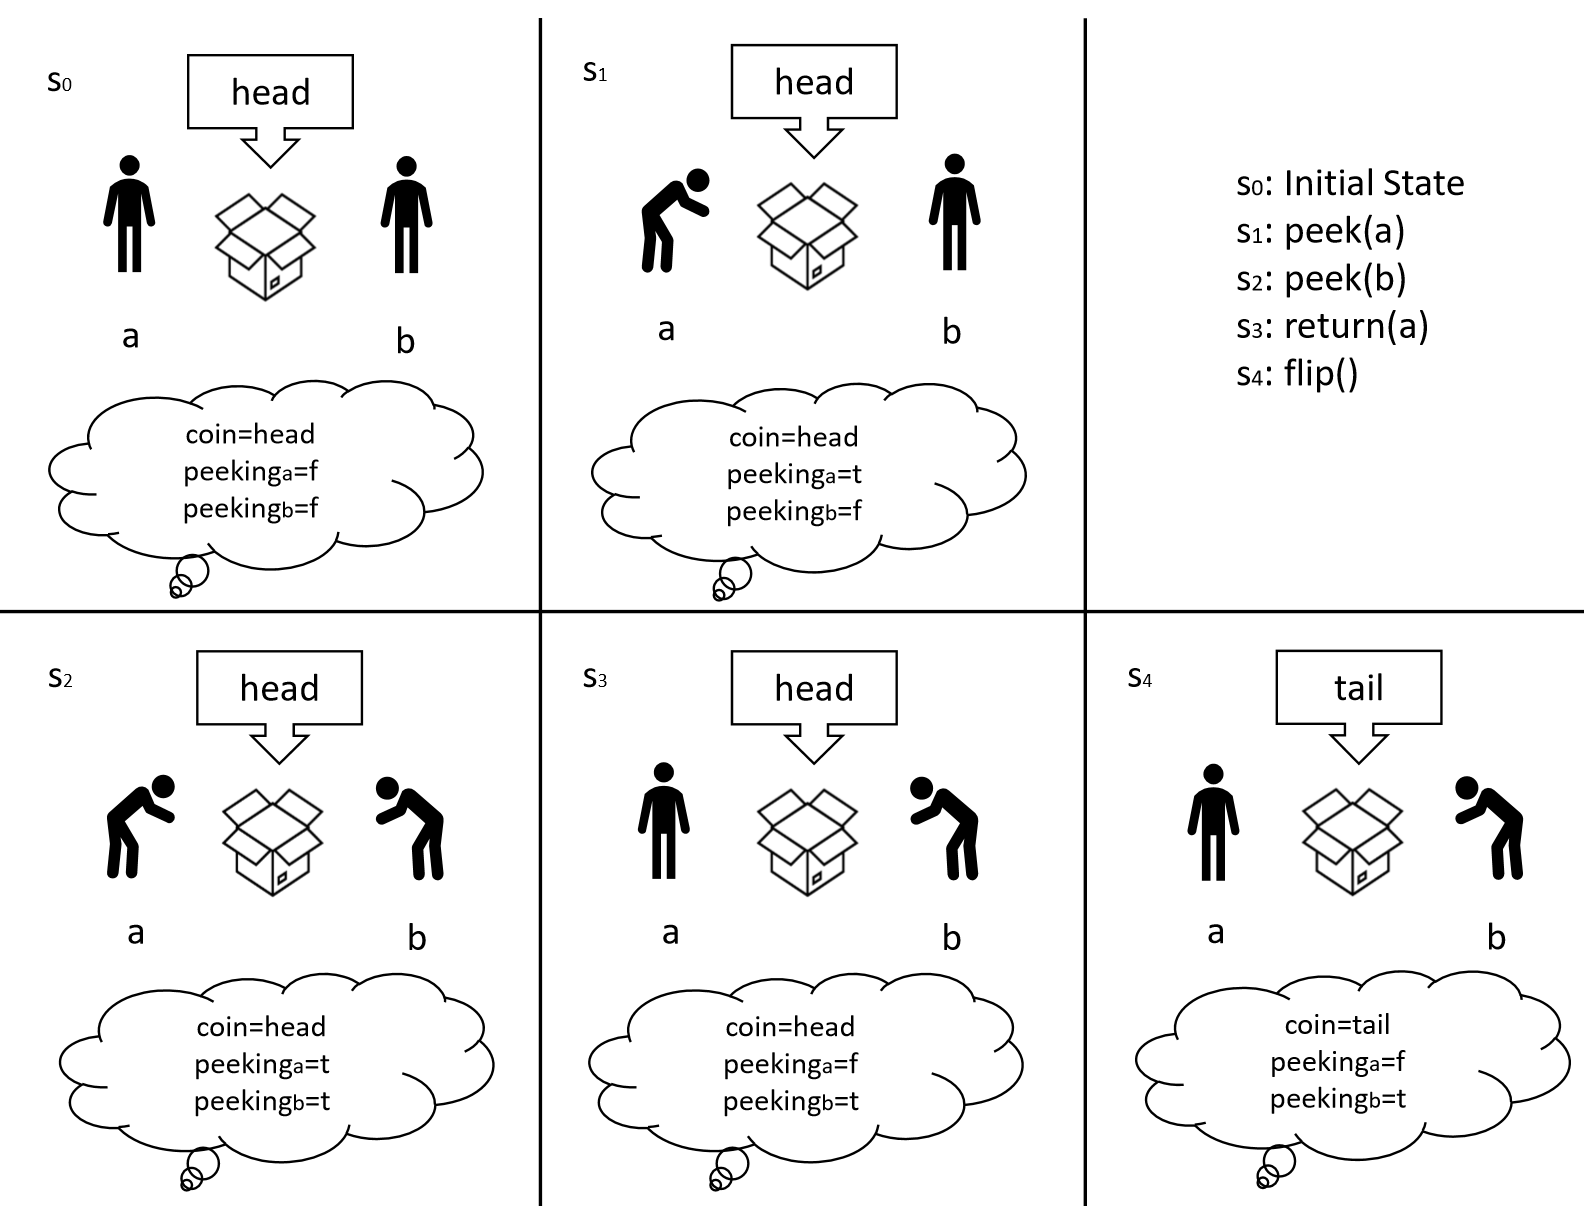
\includegraphics[width=0.9\columnwidth]{Figures/coin_plan1_s.png}
%     \caption{ The sequence of states for Plan~\ref{plan1}}
%     \label{fig:coin_plan1_s}
% \end{figure}



% Using the same example from Example~\ref{example:coin}, the state sequence $\seq=[s_0,s_1,s_2,s_3,s_4]$ from Figure~\ref{fig:coin_plan1_s} can be represented as follows:
% \begin{itemize}
%     \item [$s_0$:] $\{peeking_a \mapsto f,\ peeking_b \mapsto f,\ coin \mapsto head\}$
%     \item [$s_1$:] $\{peeking_a \mapsto t,\ peeking_b \mapsto f,\ coin \mapsto head\}$
%     \item [$s_2$:] $\{peeking_a \mapsto t,\ peeking_b \mapsto t,\ coin \mapsto head\}$
%     \item [$s_3$:] $\{peeking_a \mapsto f,\ peeking_b \mapsto t,\ coin \mapsto head\}$
%     \item [$s_4$:] $\{peeking_a \mapsto f,\ peeking_b \mapsto t,\ coin \mapsto tail\}$
% \end{itemize}

% \begin{figure}
%     \centering
%     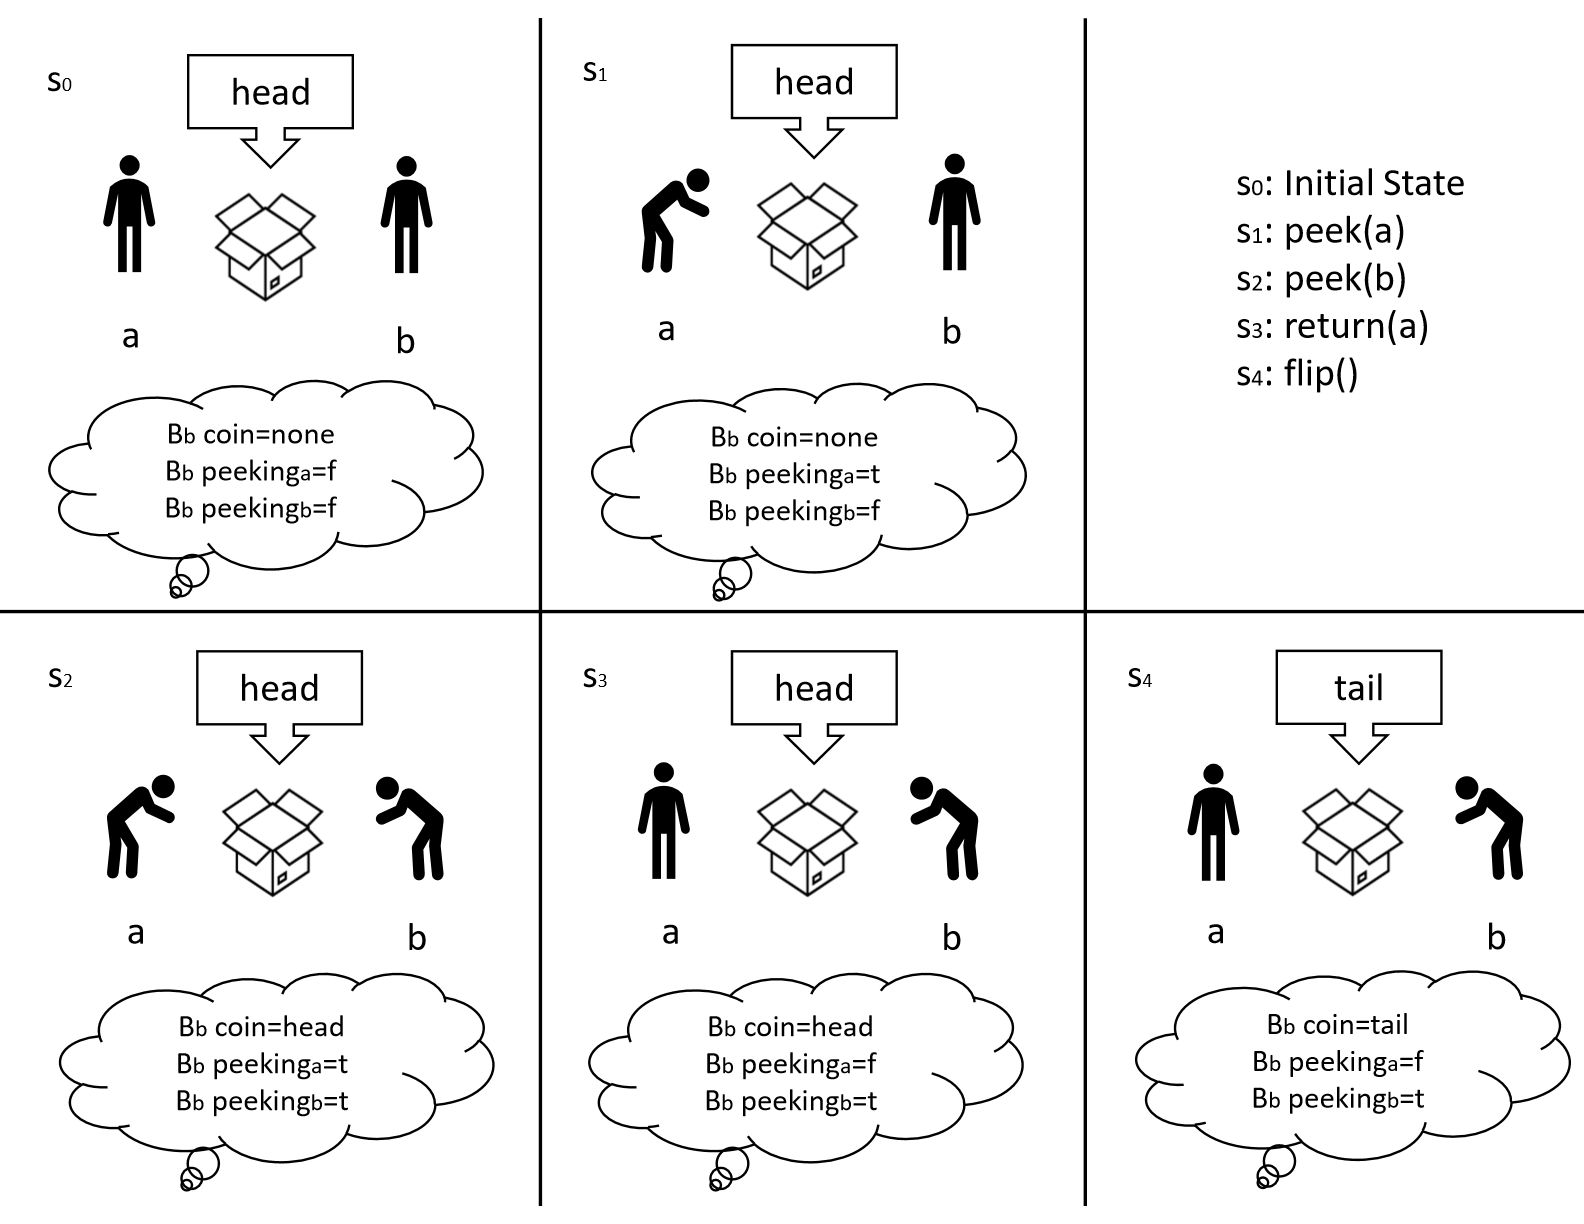
\includegraphics[width=0.9\columnwidth]{Figures/coin_plan1_sb.png}
%     \caption{ Agent $b$'s perspective for Plan~\ref{plan1}}
%     \label{fig:coin_plan1_sb}
% \end{figure}



% Agent $b$'s perspectives ($\f_b(\seq)$) should be (Figure~\ref{fig:coin_plan1_sb}):
% \begin{itemize}
%     \item [$s_0$:] $\{peeking_a \mapsto f,\ peeking_b \mapsto f,\ coin \mapsto None\}$
%     \item [$s_1$:] $\{peeking_a \mapsto t,\ peeking_b \mapsto f,\ coin \mapsto None\}$
%     \item [$s_2$:] $\{peeking_a \mapsto t,\ peeking_b \mapsto t,\ coin \mapsto head\}$
%     \item [$s_3$:] $\{peeking_a \mapsto f,\ peeking_b \mapsto t,\ coin \mapsto head\}$
%     \item [$s_4$:] $\{peeking_a \mapsto f,\ peeking_b \mapsto t,\ coin \mapsto tail\}$
% \end{itemize}
% All variables agent $b$ can see are in the red dash circles.


% \begin{figure}
%     \centering
%     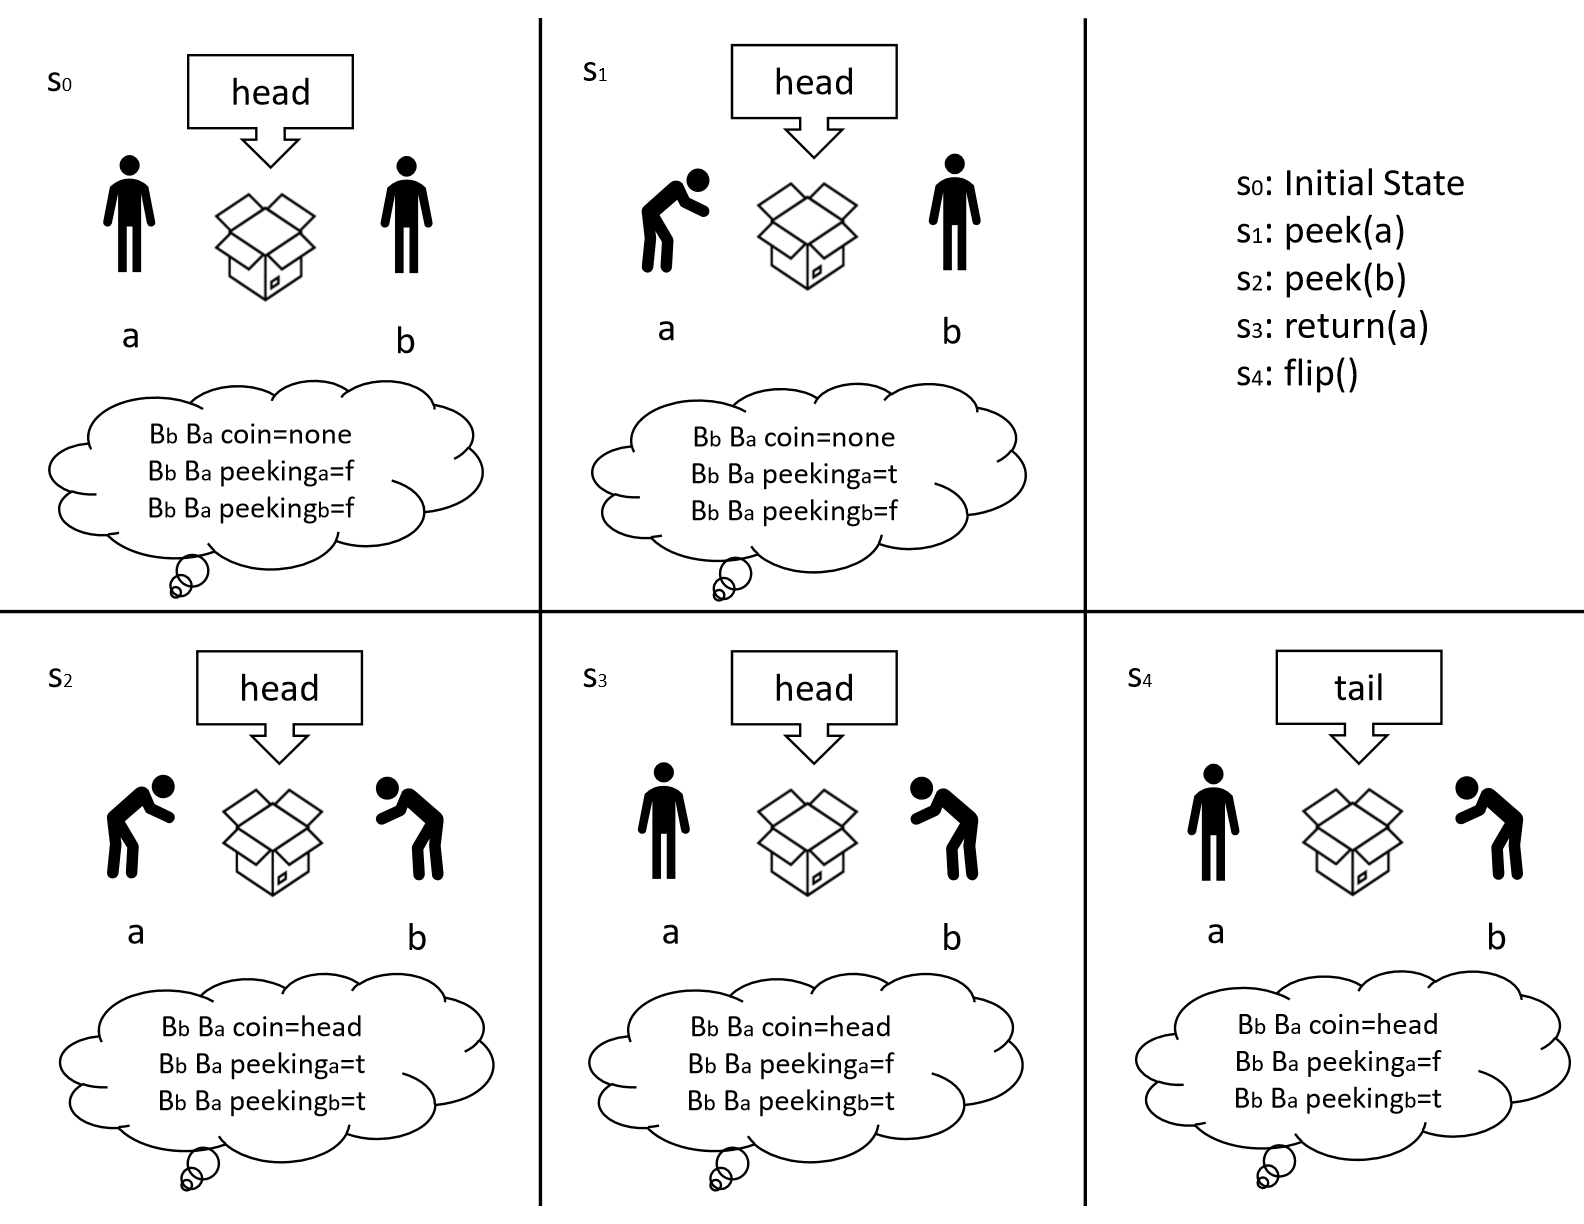
\includegraphics[width=0.9\columnwidth]{Figures/coin_plan1_sba.png}
%     \caption{ Agent $a$'s perspective under $b$'s perspective for Plan~\ref{plan1}}
%     \label{fig:coin_plan1_sba}
% \end{figure}

% In agent $b$'s mind, agent $a$'s perspectives ($\f_a(\f_b(\seq))$) should be (Figure~\ref{fig:coin_plan1_sba}):
% \begin{itemize}
%     \item [$s_0$:] $\{peeking_a \mapsto f,\ peeking_b \mapsto f,\ coin \mapsto None\}$
%     \item [$s_1$:] $\{peeking_a \mapsto t,\ peeking_b \mapsto f,\ coin \mapsto None\}$
%     \item [$s_2$:] $\{peeking_a \mapsto t,\ peeking_b \mapsto t,\ coin \mapsto head\}$
%     \item [$s_3$:] $\{peeking_a \mapsto f,\ peeking_b \mapsto t,\ coin \mapsto head\}$
%     \item [$s_4$:] $\{peeking_a \mapsto f,\ peeking_b \mapsto t,\ coin \mapsto head\}$
% \end{itemize}

% \begin{figure*}
%     \centering
%     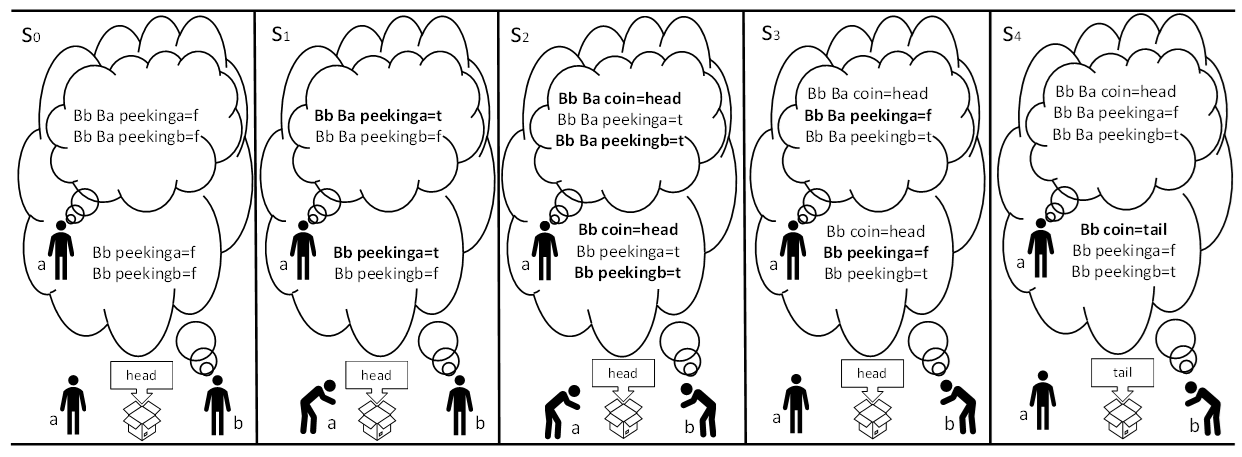
\includegraphics[width=0.9\textwidth]{Figures/plan_1_final.png}
%     \caption{Plan~\ref{plan1} with agent $b$'s justified beliefs. Bold text indicates belief that has changed.}
%     \label{fig:plan_1_final}
% \end{figure*}

Figure~\ref{fig:plan_1_final} shows the evolution of agent $b$'s justified perspective as well as agent $b$'s mind about agent $a$'s justified perspective.
Since agent $b$'s justified perspectives are derived directly from the sequence of world states $\seq$, $b$'s justified perspectives are generated simply based on $b$'s observation function.
However, the nested perspective $\f_a(\f_b(\seq))$ is worth discussing.
As both $peeking_a$ and $peeking_b$ are visible to all agents at all times, they are always common knowledge. We focus on the steps needed to retrieve the value for variable $coin$ in state $s_4$ to generate $\f_a(\f_b(\seq))$:

\begin{enumerate}
    \item Under $b$'s justified perspective $\f_b(\seq)$, finding all the timestamps ($a\timestamp$) that agent $a$ sees $coin$. The set of timestamps $ts = \{1,2\}$.
    \item Identifying the latest timestamp ($lt$) that agent $a$ sees $coin$ in $\f_b(\seq)$, which is $2$. 
    \item  $\memorization(\f_b(\seq),2,coin) = \f_b(\seq)[2](coin)=head$ since $coin\in \f_b(\seq)[2]$ and $b$'s perspective of $coin$ at this time is $head$.. 
\end{enumerate}
\end{example}

\end{comment}

\begin{example}[Example~\ref{example:coin} with Plan~\ref{plan2}]

% \begin{figure}
%     \centering
%     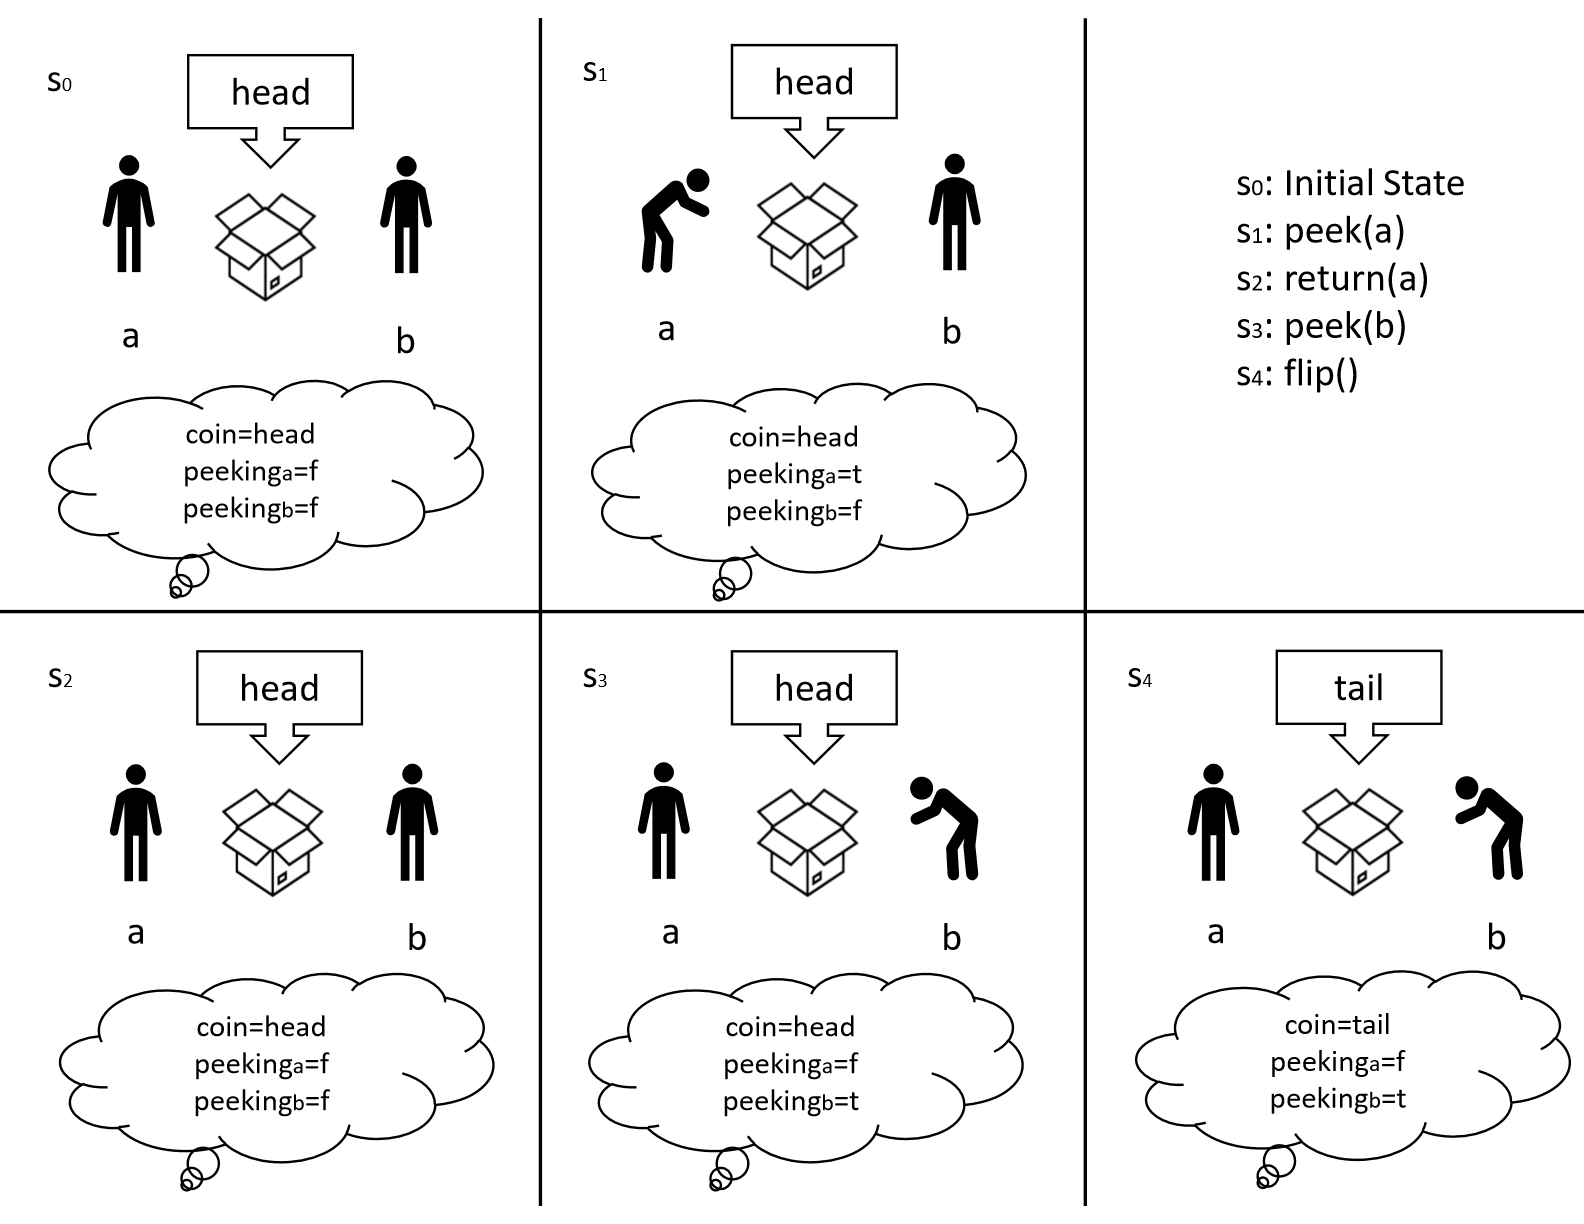
\includegraphics[width=0.9\columnwidth]{Figures/coin_plan2_s.png}
%     \caption{The sequence of states for Plan~\ref{plan2}}
%     \label{fig:coin_plan2_s}
% \end{figure}

% Let the sequence of states generated by this plan as $\seq = s_0,s_1,s_2,s_3,s_4$ (shown in Figure~\ref{fig:coin_plan2_s}).


% \begin{figure}
%     \centering
%     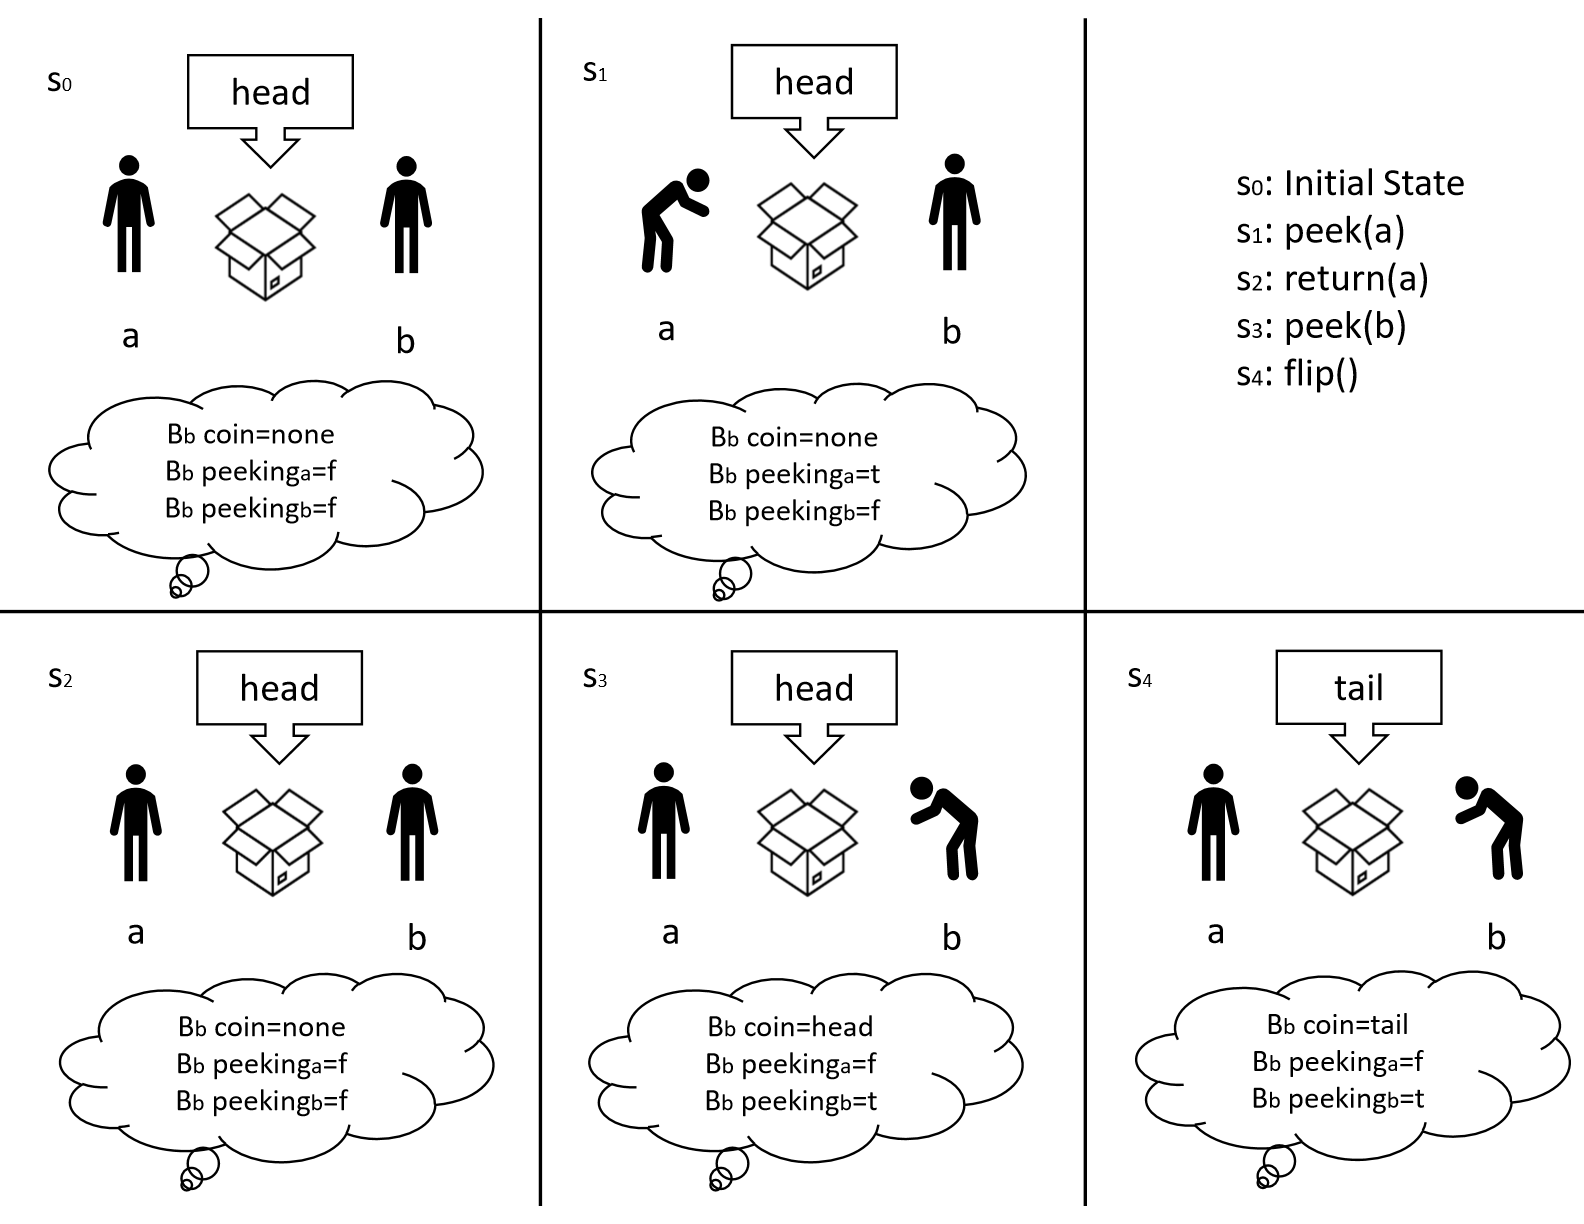
\includegraphics[width=0.9\columnwidth]{Figures/coin_plan2_sb.png}
%     \caption{ Agent $b$'s perspective for Plan~\ref{plan2}}
%     \label{fig:coin_plan2_sb}
% \end{figure}



% Agent $b$'s perspectives $\f_b(\seq)$ (shown in Figure~\ref{coin_plan2_sb}) should be:
% \begin{itemize}
%     \item [$s_0$:] $\{peeking_a \mapsto f,\ peeking_b \mapsto f,\ coin \mapsto None\}$
%     \item [$s_1$:] $\{peeking_a \mapsto t,\ peeking_b \mapsto f,\ coin \mapsto None\}$
%     \item [$s_2$:] $\{peeking_a \mapsto f,\ peeking_b \mapsto f,\ coin \mapsto None\}$
%     \item [$s_3$:] $\{peeking_a \mapsto f,\ peeking_b \mapsto t,\ coin \mapsto head\}$
%     \item [$s_4$:] $\{peeking_a \mapsto f,\ peeking_b \mapsto t,\ coin \mapsto tail\}$
% \end{itemize}

% \begin{figure}
%     \centering
%     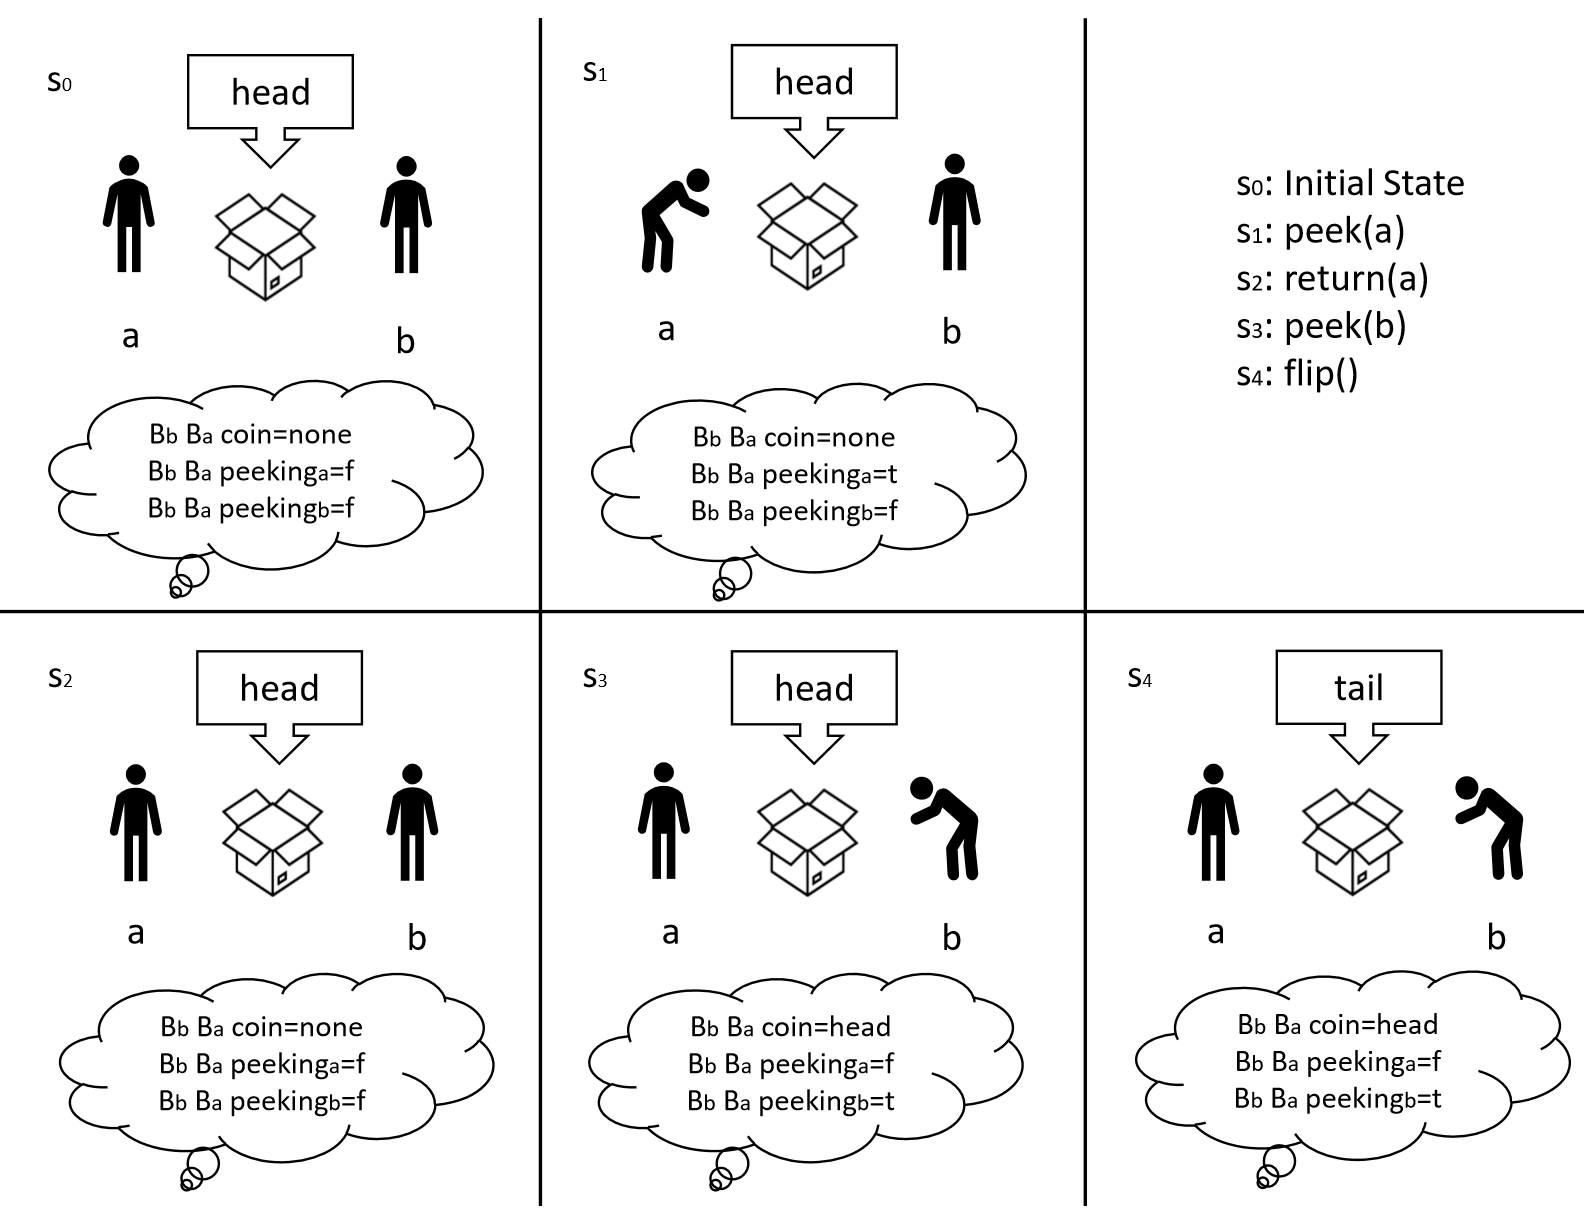
\includegraphics[width=0.9\columnwidth]{Figures/coin_plan2_sba.png}
%     \caption{ Agent $a$'s perspective under $b$'s perspective for Plan~\ref{plan2}}
%     \label{fig:coin_plan2_sba}
% \end{figure}



% In agent $b$'s mind, agent $a$'s perspectives $\f_a(\f_b(\seq))$ (shown in Figure~\ref{fig:coin_plan2_sb}) should be:
% \begin{itemize}
%     \item [$s_0$:] $\{peeking_a \mapsto f,\ peeking_b \mapsto f,\ coin \mapsto None\}$
%     \item [$s_1$:] $\{peeking_a \mapsto t,\ peeking_b \mapsto f,\ coin \mapsto None\}$
%     \item [$s_2$:] $\{peeking_a \mapsto f,\ peeking_b \mapsto f,\ coin \mapsto None\}$
%     \item [$s_3$:] $\{peeking_a \mapsto f,\ peeking_b \mapsto t,\ coin \mapsto head\}$
%     \item [$s_4$:] $\{peeking_a \mapsto f,\ peeking_b \mapsto t,\ coin \mapsto head\}$
% \end{itemize}

% \tm{I think what you have illustrated in the figures is very nice; but you need to do something other than use colours. Some people print in black and white; some are heavily colourblind. Why not just have this figure once and write $B_a coin=head$, etc. under each agent in each state? That will take up a similar amount of room, but then the beliefs, including nested beliefs, will be explicit and easy to understand}
% \gh{Updated}
% \begin{figure}
%     \centering
%     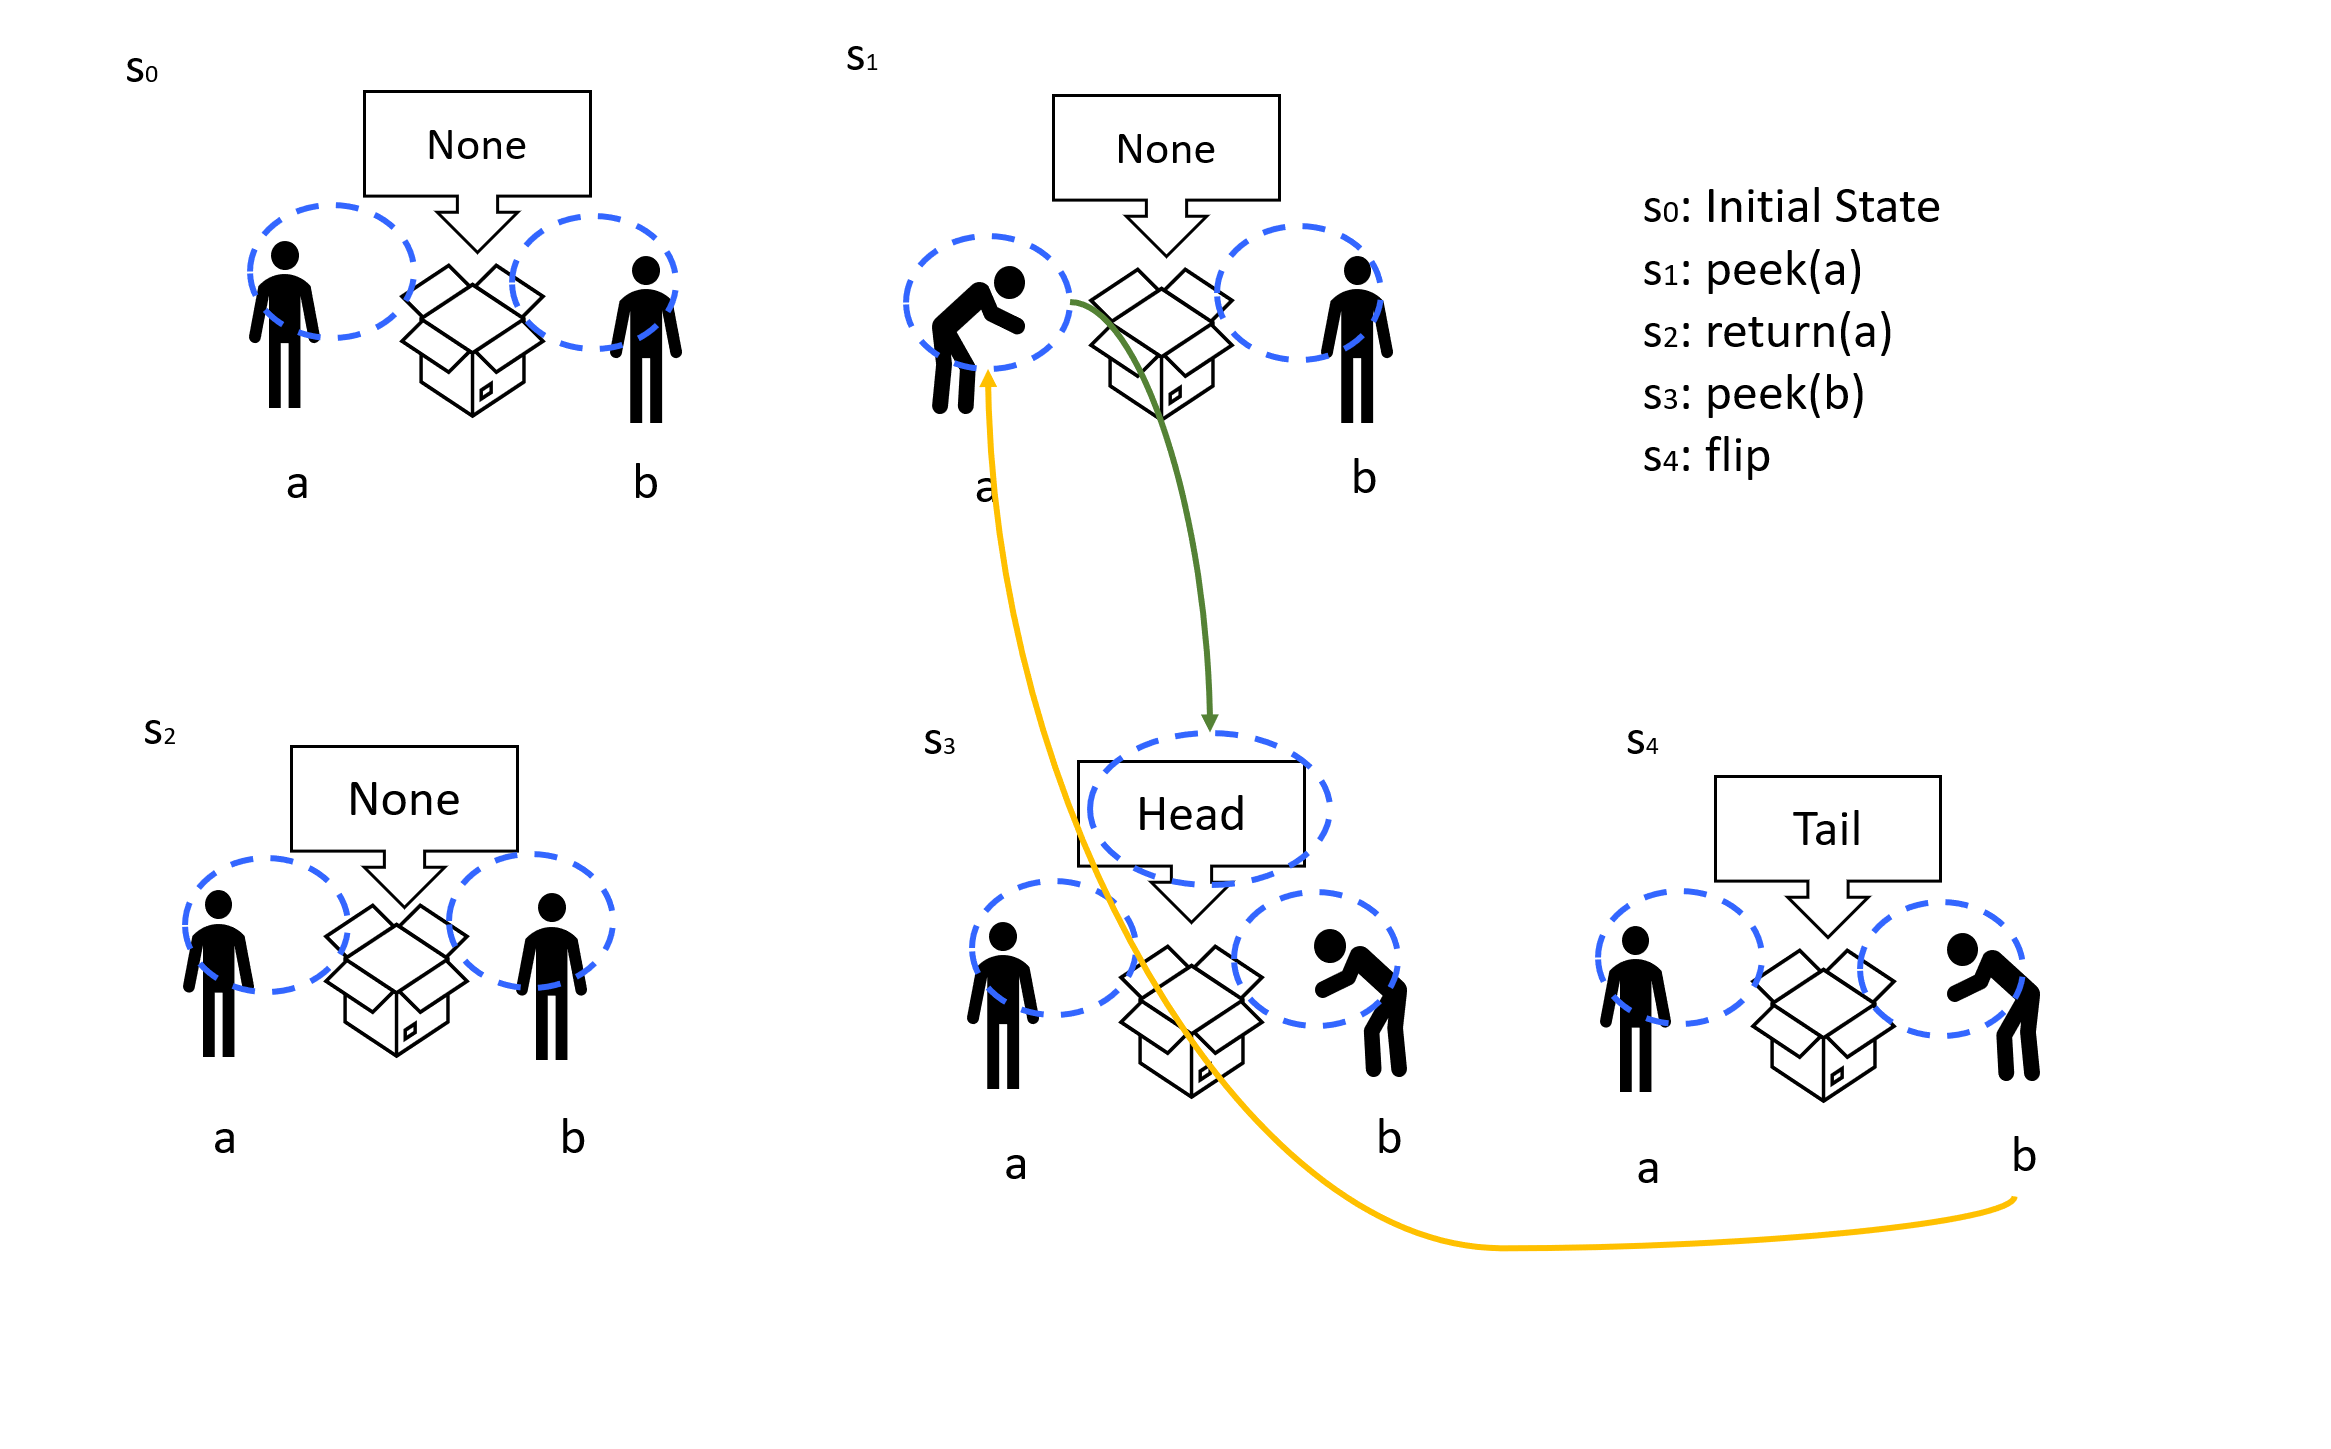
\includegraphics[width=0.9\columnwidth]{Figures/coin_example_2_ba.png}
%     \caption{ Agent $a$'s perspective under agent $b$'s perspective }
%     \label{fig:coin_example2_ba}
% \end{figure}

% \begin{figure*}
%     \centering
%     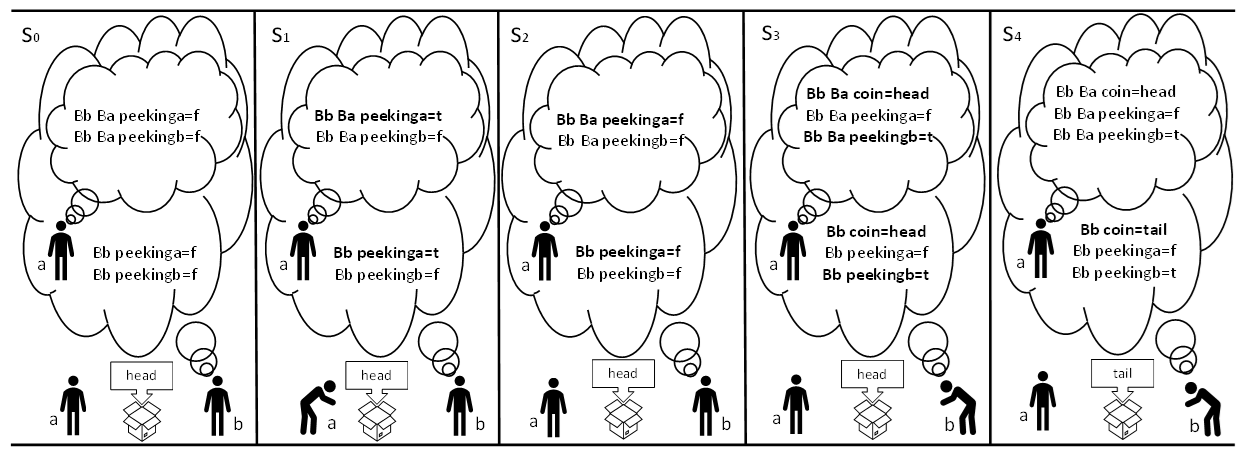
\includegraphics[width=0.9\textwidth]{Figures/plan_2_final.png}
%     \caption{Plan~\ref{plan2} with agent $b$'s justified beliefs. Bold text indicates belief that has changed.}
%     \label{fig:plan_2_final}
% \end{figure*}


In Figure~\ref{fig:plan_2_final}, agent $b$ cannot at the same time: 1) see agent $a$ peeking into the box and 2) see what was inside the box at that time, because $a$ and $b$ are no longer peeking into the box at the same time, as they were in $s_2$ from Plan~\ref{plan1}.
The latest timestamp $lt$ agent $a$ peeked into the box is $1$.
We can retrieve the value of the $coin$ at timestamp 1 from $b$'s perspective using $\memorization(\seq,1,coin)$.
In agent $b$'s perspective, there is no information about $coin$ until $s_3$, making the return value of $\memorization(\seq,1,coin)$ to be $\f_b(s)[3](coin)=head$.
% In agent $b$'s perspective, there is no information about $coin$ until $s_3$, so in $\memorization(\seq,1,coin)$, we have that the value of $coin$ is $head$ in $\f_b(\seq)$ at timestamp $3$.
So, $M,\seq \vDash B_b B_a coin=head$ is equivalent to $M,\f_b(\seq) \vDash B_a coin=head $, which is $M,\f_a(\f_b(\seq)) \vDash coin=head$.
Therefore, the justified belief of agent $b$ on a false belief about agent $a$ on $\varphi$ can be generated even if $b$ cannot see both 1) the truth value of $\varphi$ while 2) seeing agent $a$ seeing $\varphi$ at the same timestamp (same state).
\end{example}








% \subsection{BBL}
% BBL is a domain that contains stationary cameras that can turn or observe a certain range in a 2-dimension plane. Let there be two agents (cameras) $a$, $b$, and one movable proposition $p$. Initially ($s_0$), both $a$ can see both $b$ and $p$, while $b$ can see only $p$.

% \begin{figure*}[ht]
%     \centering
%     % % \begin{tikzpicture}
% %   \matrix (m) [matrix of math nodes,row sep=3em,column sep=4em,minimum width=2em]
% %   {
% %      F_t(x) & F(x) \\
% %      A_t & A \\};
% %   \path[-stealth]
% %     (m-1-1) edge node [left] {$\mathcal{B}_X$} (m-2-1)
% %             edge [double] node [below] {$\mathcal{B}_t$} (m-1-2)
% %     (m-2-1.east|-m-2-2) edge node [below] {$\mathcal{B}_T$}
% %             node [above] {$\exists$} (m-2-2)
% %     (m-1-2) edge node [right] {$\mathcal{B}_T$} (m-2-2)
% %             edge [dashed,-] (m-2-1);
% % \end{tikzpicture}


% \newcommand{\scale}{0.4}
% \newcommand{\range}{30}
% \newcommand{\size}{3}
% \newcommand{\oversize}{6}
% \makeatletter
% \newcommand{\gettikzxy}[3]{%
%   \tikz@scan@one@point\pgfutil@firstofone#1\relax
%   \edef#2{\the\pgf@x}%
%   \edef#3{\the\pgf@y}%
% }
% \makeatother

% \begin{tikzpicture}
%     \coordinate (top_left) at (0,20*\scale);
%     \coordinate (bottom_left) at (0,0);
%     \coordinate (top_right) at (20*\scale,20*\scale);
%     \coordinate (bottom_right) at (20*\scale,0);

%     \coordinate (origin) at (0,0);
%     \coordinate (a1) at (5*\scale,5*\scale);
%     \coordinate (a1_up) at (5*\scale,20*\scale);
%     \coordinate (a1_down) at (20*\scale,5*\scale);
%     \coordinate (a1_dir) at (6*\scale,6*\scale);
%     \coordinate (a2) at (15*\scale,15*\scale);
%     \coordinate (a2_up) at (0,15*\scale);
%     \coordinate (a2_down) at (15*\scale,0);
%     \coordinate (a2_dir) at (14*\scale,14*\scale);
        
%     \begin{scope}[transparency group]
%         \begin{scope}[blend mode=multiply]
%             \fill[ opacity=0.5,blue!30] (a1) -- (a1_up) -- (top_right) -- (a1_down) -- cycle;
%             \fill[ opacity=0.5,yellow!30] (a2) -- (a2_up) -- (bottom_left) -- (a2_down) -- cycle;
%         \end{scope}
%     \end{scope}
    
%     \draw[thick, black,->] (a1) -- (a1_dir);
%     \draw[thick, black,->] (a2) -- (a2_dir);
    

%     \draw[thick] let    \p{1} = (a1)    in (a1 |- origin)
%         node[circle,fill=red!80,inner sep=2pt,
%         label={[align=center]below:
%                 $a_1$ \\ 
%                 (\pgfmathparse{(\x1/28.45274)}\num[round-mode=places,round-precision=1]{\pgfmathresult},
%                 \pgfmathparse{(\y1/28.45274)}\num[round-mode=places,round-precision=1]{\pgfmathresult})
%                 }] at (\x1,\y1) {};
%     \draw[->, black] (a1) -- (a1_up);
%     \draw[->, black] (a1) -- (a1_down);
    
                
%     \draw[thick] let    \p{1} = (a2)    in (a1 |- origin)
%         node[circle,fill=red!80,inner sep=2pt,
%         label={[align=center]below:
%                 $a_2$ \\ 
%                 (\pgfmathparse{(\x1/28.45274)}\num[round-mode=places,round-precision=1]{\pgfmathresult},
%                 \pgfmathparse{(\y1/28.45274)}\num[round-mode=places,round-precision=1]{\pgfmathresult})
%                 }] at (\x1,\y1) {};
%     \draw[->, black] (a2) -- (a2_up);
%     \draw[->, black] (a2) -- (a2_down);
    
    
%     % border

    
%     \draw[black] (top_left) -- (bottom_left) -- (bottom_right) -- (top_right) -- cycle;

    
%     % \draw[->, gray, thick] ({cos(\range)*\size*2},0) -- ({cos(\range)*\size*2-cos(\range)*\oversize},{sin(\range)*\oversize});
%     % \draw[->, gray, thick] ({cos(\range)*\size*2},0) -- ({cos(\range)*\size*2},0) -- ({cos(\range)*\size*2-cos(\range)*\oversize},-{sin(\range)*\oversize});
    
    
%     \coordinate (b1) at (10*\scale,10*\scale);
%     \coordinate (b2) at (2.5*\scale,2.5*\scale);
%     \coordinate (b3) at (17.5*\scale,17.5*\scale);
    
%     \draw[thick] let    \p{1} = (b1)    in (a1 |- origin)
%         node[circle,fill=black!80,inner sep=1pt,
%         label={[align=center]below:
%                 $b_1$ \\ 
%                 (\pgfmathparse{(\x1/28.45274)}\num[round-mode=places,round-precision=1]{\pgfmathresult},
%                 \pgfmathparse{(\y1/28.45274)}\num[round-mode=places,round-precision=1]{\pgfmathresult})
%                 }] at (\x1,\y1) {};
                
%     \draw[thick] let    \p{1} = (b2)    in (a1 |- origin)
%         node[circle,fill=black!80,inner sep=1pt,
%         label={[align=center]below:
%                 $b_2$ \\ 
%                 (\pgfmathparse{(\x1/28.45274)}\num[round-mode=places,round-precision=1]{\pgfmathresult},
%                 \pgfmathparse{(\y1/28.45274)}\num[round-mode=places,round-precision=1]{\pgfmathresult})
%                 }] at (\x1,\y1) {};    

%     \draw[thick] let    \p{1} = (b3)    in (a1 |- origin)
%         node[circle,fill=black!80,inner sep=1pt,
%         label={[align=center]below:
%                 $b_3$ \\ 
%                 (\pgfmathparse{(\x1/28.45274)}\num[round-mode=places,round-precision=1]{\pgfmathresult},
%                 \pgfmathparse{(\y1/28.45274)}\num[round-mode=places,round-precision=1]{\pgfmathresult})
%                 }] at (\x1,\y1) {};    
                
%     % \filldraw[black] ({cos(\range)*\size},0) circle (2pt) node[anchor=west] {$b_2$};
%     % \filldraw[black] (-{cos(\range)*\size},0) circle (2pt) node[anchor=west] {$b_1$};
%     % \filldraw[black] ({cos(\range)*\size*3},0) circle (2pt) node[anchor=west] {$b_3$};
%     % \filldraw[black] ({cos(\range)*\size},{sin(\range)*\oversize*3/4}) circle (2pt) node [anchor=west] {$b_4$};
    

    
    
%     % border
%     % \draw[gray, thick] (-{cos(\range)*\size*2},-{sin(\range)*\oversize}) -- ({cos(\range)*\size*4},-{sin(\range)*\oversize});
%     % \draw[gray, thick] (-{cos(\range)*\size*2},{sin(\range)*\oversize}) -- ({cos(\range)*\size*4},{sin(\range)*\oversize});
%     % \draw[gray, thick] ({cos(\range)*\size*4},{sin(\range)*\oversize}) -- ({cos(\range)*\size*4},-{sin(\range)*\oversize});
%     % \draw[gray, thick] (-{cos(\range)*\size*2},{sin(\range)*\oversize}) -- (-{cos(\range)*\size*2},-{sin(\range)*\oversize});
% \end{tikzpicture}

% % \begin{tikzpicture}
% %     %\draw [help lines] (0,0) grid (4,4);
% %     %\coordinate (origin) at (0,0);
% %     \node[circle,fill]  (d1) at (3,2) {};

% %     %\draw[red,thick] let    \p{1} = (d1)    in (d1|- origin) node[label=below:$\x1$]{} --  (d1) --  (d1 -| origin) node[label=left:\y1]{} ;

% %     \end{tikzpicture}




% \begin{tikzpicture}
%   \matrix (m) [matrix of math nodes,row sep=3em,column sep=4em,minimum width=2em]
%   {
%      F_t(x) & F(x) \\
%      A_t & A \\};
%   \path[-stealth]
%     (m-1-1) edge node [left] {$\mathcal{B}_X$} (m-2-1)
%             edge [double] node [below] {$\mathcal{B}_t$} (m-1-2)
%     (m-2-1.east|-m-2-2) edge node [below] {$\mathcal{B}_T$}
%             node [above] {$\exists$} (m-2-2)
%     (m-1-2) edge node [right] {$\mathcal{B}_T$} (m-2-2)
%             edge [dashed,-] (m-2-1);
% \end{tikzpicture}


\newcommand{\scale}{0.4}
\newcommand{\range}{30}
\newcommand{\size}{3}
\newcommand{\oversize}{6}
\makeatletter
\newcommand{\gettikzxy}[3]{%
  \tikz@scan@one@point\pgfutil@firstofone#1\relax
  \edef#2{\the\pgf@x}%
  \edef#3{\the\pgf@y}%
}
\makeatother

\begin{tikzpicture}
    \coordinate (top_left) at (0,20*\scale);
    \coordinate (bottom_left) at (0,0);
    \coordinate (top_right) at (20*\scale,20*\scale);
    \coordinate (bottom_right) at (20*\scale,0);

    \coordinate (origin) at (0,0);
    \coordinate (a1) at (10*\scale,10*\scale);
    \coordinate (a1_up) at (0*\scale,10*\scale);
    \coordinate (a1_down) at (10*\scale,0*\scale);
    \coordinate (a1_opp) at (0*\scale,0*\scale);
    
    \coordinate (a1_dir) at (9*\scale,9*\scale);
    
    \coordinate (a2) at (15*\scale,15*\scale);
    \coordinate (a2_up) at (0,15*\scale);
    \coordinate (a2_down) at (15*\scale,0);
    \coordinate (a2_dir) at (14*\scale,14*\scale);
    

    \coordinate (b2) at (5*\scale,5*\scale);
    
        
    \begin{scope}[transparency group]
        \begin{scope}[blend mode=multiply]
            \fill[ opacity=0.5,blue!30] (a1) -- (a1_up) -- (a1_opp) -- (a1_down) -- cycle;
            \fill[ opacity=0.5,yellow!30] (a2) -- (a2_up) -- (bottom_left) -- (a2_down) -- cycle;
        \end{scope}
    \end{scope}
    
    \draw[thick, black,->] (a1) -- (a1_dir);
    \draw[thick, black,->] (a2) -- (a2_dir);
    

    \draw[thick] let    \p{1} = (a1)    in (a1 |- origin)
        node[circle,fill=red!80,inner sep=2pt,
        label={[align=center, xshift=0.6cm]below:
                $b$ \\ 
                (10,10)
                }] at (\x1,\y1) {};
    \draw[->, black] (a1) -- (a1_up);
    \draw[->, black] (a1) -- (a1_down);
    
                
    \draw[thick] let    \p{1} = (a2)    in (a1 |- origin)
        node[circle,fill=red!80,inner sep=2pt,
        label={[align=center, xshift=0.5cm]below:
                $a$ \\ 
                (15,15)
                }] at (\x1,\y1) {};
    \draw[->, black] (a2) -- (a2_up);
    \draw[->, black] (a2) -- (a2_down);
    
    
    % border

    
    \draw[black] (top_left) -- (bottom_left) -- (bottom_right) -- (top_right) -- cycle;
    
    

    
                
    \draw[thick] let    \p{1} = (b2)    in (a1 |- origin)
        node[circle,fill=black!80,inner sep=1pt,
        label={[align=center]above:
                $c$ \\ 
                (5,5)
                }] at (\x1,\y1) {};    

                
\end{tikzpicture}

%     \caption{Example for Big Brother Logic}
%     \label{fig:big_brother_exp}
% \end{figure*}

% \subsubsection{Initial State}
% Firstly, in order to model this domain into state, we need to have variables that represents the directions of the agents: $dir(a)$ and $dir(b)$, and the location of the proposition $loc(p)$. Since all agents are stationary, with the information of the direction, it is easy to calculate whether an agent can see something or not based on the line of sight in the perspective functions. Then, initially, the global state and agent's local state should be $\{dir(a),dir(b),loc(p),p\}$, $\{dir(a),dir(b),loc(p),p\}$ and $\{dir(a)=null,dir(b),loc(p),p\}$ respectively. And clearly, we have the following epistemic relations:
% \begin{itemize}
%     \item $K_a p$, $K_b p$
%     \item $K_a K_b p$, $\neg K_b K_a p$ ($\neg S_b S_a p$)
%     \item $B_a p$, $B_b p$
%     \item $K_a B_b p$, $\neg K_b B_a p$
%     \item $B_a B_b p$, $\neg B_b B_a p$
% \end{itemize}

% \subsubsection{State 1}
% Then, we rotate the direction of the agent $b$ by $180_{\circ} $ so that he could see $a$, but cannot see $p$. We note this state as $s1$ and $b$'s direction as $dir(b)'$. Then, we have each agents observation as $\{dir(a),dir(b)',loc(p),p\}$ and $\{dir(b)',dir(a)\}$ respectively. In the meantime, $\memorization_b(s_1)$ = $\f_b(s_0) \backslash \observation_b(s_1) = \{loc(p),p\}$.
% Based on their perspectives, we have:

% \begin{itemize}
%     \item $K_a p$, $\neg K_b p$
%     \item $K_a \neg K_b p$ ($K_a \neg S_b p$), $\neg K_b K_a p$ ($\neg S_b p$)
%     \item $B_a p$, $B_b p$
%     \item $K_a B_b p$, $\neg K_b B_a p$ ($\neg S_b p$)
%     \item $B_a B_b p$, $B_b B_a p$
% \end{itemize}

% Most of the above epistemic formulae are trivial, except $\neg K_b B_a p$, $B_b B_a p$ and $B_a B_b p$. For agent $b$, in order to see $B_a p$, he need to see all the variables that related to the evaluation of the formula, which includes $p$ and $dir(a)$. Since $\neg S_b p$, then we have $\neg K_b B_a p$. 
% As for $B_b B_a p$, $(M,s_1) \vDash B_b B_a p$ holds when $(M,\f_b(s_1)) \vDash B_a p$, which means $(M,\f_a(\f_b(s_1))) \vDash p$.
% In $b$'s perspective of the world $s_1$, we have $\{dir(b)',dir(a),loc(p),p\}$ and $a$'s prespective about this would be $\{dir(b)',dir(a),loc(p),p\}$, which holds $(M,\f_a(\f_b(s_1))) \vDash p$.
% As for $B_a B_b p$, it is a bit trickier. 
% $(M,s_1) \vDash B_a B_b p$ holds when $(M,\f_a(s_1)) \vDash B_b p$, which is equivalent $(M,\f_b(\f_a(s_1))) \vDash p$. Then, in $a$'s perspective ($\{dir(a),dir(b)',loc(p),p\}$) of the world $s1$, $b$'s perspective cannot be calculated with ease. 
% Firstly, we induct $b$'s observation over a's perspective of $s1$: $\observation_b(\f_a(s_1)) = \{dir(b)'\}$. 
% Then, we need to figure out $b$'s perspective of the previous timestamp ($\f_a(s_0)$), we have $\f_a(s_0) = \{dir(a),dir(b),loc(p),p\}$ and $\f_b(\f_a(s_0))=\{dir(a),dir(b),loc(p),p\}$.
% At last, we can calculated $\memorization_b(\f_a(s_1)) = \{dir(a),dir(b),loc(p),p\}$ to form $\f_b(\f_a(s_1))=\{dir(a),dir(b),loc(p),p,dir(b)'\}$
% Then, we can find out that the $(M,s_1) \vDash B_a B_b p$ holds.

% \gh{It is interested to evaluate $B_a S_b S_c p$, should it be true or not?}

% \subsubsection{State 2}
% Then, we change the value of the $p$ to $\neg p$ to generate false belief and note this state as $s_2$. Now, each agent's observation becomes $\{dir(a),dir(b)',loc(p),\neg p\}$, $\{dir(b)',dir(c)\}$ and $\{dir(a),dir(b)',dir(c),loc(p),\neg p\}$, respectively. In the meantime, $\memorization_b(s_1)$ = $\f_b(s_1) \backslash \observation_b(s_1) = \{dir(a),loc(p),p\}$.

% \begin{itemize}
%     \item $K_a \neg p$, $\neg K_b \neg p$, $K_c \neg p$
%     \item $K_a \neg K_b \neg p$ ($K_a \neg S_b \neg p$), $\neg K_b K_a \neg p$ ($\neg S_b \neg p$), $K_c K_a \neg p$, $K_c K_b \neg p$ ($K_c \neg S_b \neg p$)
%     \item $B_a \neg p$, $B_b p$, $B_c \neg p$
%     \item $K_a B_b p$, $\neg K_b B_a \neg p$ ($\neg S_b \neg p$), $K_c B_a \neg p$, $K_c B_b p$, $\neg K_a B_c \neg p$, $\neg K_b B_c \neg p$ ($\neg S_b \neg p$)
%     \item $B_a B_b p$, $B_b B_a p$, $B_c B_a \neg p$, $B_c B_b p$, $\neg B_a B_c \neg p$, $B_b B_c p$
% \end{itemize}

% Now, the epistemic formulae are harder to evaluate. $M,s_2 \vDash K_a B_b p$ is equivalent to $ M,s_2 \vDash S_a B_b p \land B_b p$. 
% $ M,s_2 \vDash B_b p$ is trivial and $ M,s_2 \vDash S_a B_b p$ is equivalent to $ M,O_a(s_2) \vDash B_b p$ is also trivial referring to the definition (e).

% Under $a$'s perspective $\{dir(a),dir(b)',dir(c),loc(p),\neg p, loc(c)=null\}$, we can get $b$'s perspective by union $b$'s observation $\{dir(b)',dir(c)=\neg null\}$ with $\memorization_b(\f_a(s_2))$ $=$ $\f_b(\f_a(s_1)) \backslash \observation_b(\f_a(s_2))$ $ = $ $\{dir(a),loc(p),p,dir(b)'\}$. 
% That gives us $ M,s_2 \vDash B_a B_b p$.

% \subsection{State 3}

% At last, we can rotate the agent $b$ to its original direction $dir(b)$ and note this state as $s_3$. 

% \begin{itemize}
%     \item $K_a \neg p$, $K_b \neg p$, $K_c \neg p$
%     \item $K_a K_b \neg p$, $ K_b K_a \neg p$, $K_c K_a \neg p$, $K_c K_b \neg p$ ($\neg S_b \neg dir(s)$)
%     \item $B_a \neg p$, $B_b \neg p$, $B_c \neg p$
%     \item $K_a B_b \neg p$, $K_b B_a \neg p$, $K_c B_a \neg p$, $K_c B_b \neg p$, $\neg K_a B_c \neg p$, $\neg K_b B_c \neg p$ ($\neg S_b \neg dir(s)$)
%     \item $B_a B_b \neg p$, $B_b B_a \neg p$, $B_c B_a \neg p$, $B_c B_b \neg p$, $\neg B_a B_c \neg p$, $B_b B_c \neg p$
% \end{itemize}

% $B_b B_c \neg p$

% BBL is a domain that contains stationary cameras that can turn or observe a certain range in a 2-dimension plane. Let there be three agents (cameras) $a$, $b$ and $c$, and one movable proposition $p$. Initially ($s_0$), both $a$ and $b$ can see $o$ and each other, while $c$ can see all of them. 


% \subsection{Example 2}

% \subsubsection{Initial State}
% Firstly, in order to model this domain into state, we need to have variables that represents the directions of the agents: $dir(a)$, $dir(b)$ and $dir(c)$, and the location of the proposition $loc(p)$. Since all agents are stationary, with the information of the direction, it is easy to calculate whether an agent can see something or not based on the line of sight in the perspective functions. Then, initially, the global state and agent's local state should be $\{dir(a),dir(b),dir(c),loc(p),p\}$, $\{dir(a),dir(b),dir(c)=null,loc(p),p\}$, $\{dir(a),dir(b),dir(c)=null,loc(p),p\}$ and $\{dir(a),dir(b),dir(c),loc(p),p\}$ respectively. And clearly, we have the following epistemic relations:
% \begin{itemize}
%     \item $K_a p$, $K_b p$, $K_c p$
%     \item $K_a K_b p$, $K_b K_a p$, $K_c K_a p$, $K_c K_b p$
%     \item $B_a p$, $B_b p$, $B_c p$
%     \item $K_a B_b p$, $K_b B_a p$, $K_c B_a p$, $K_c B_b p$, $\neg K_a B_c p$, $\neg K_b B_c p$
%     \item $B_a B_b p$, $B_b B_a p$, $B_c B_a p$, $B_c B_b p$, $\neg B_a B_c p$, $\neg B_b B_c p$
% \end{itemize}

% \subsection{State 1}
% Then, we rotate the direction of the agent $b$ so that he could see $c$, but cannot see $a$ and $p$. We note this state as $s1$ and $b$'s direction as $dir(b)'$. Then, we have each agents observation as $\{dir(a),dir(b)',loc(p),p\}$, $\{dir(b)',dir(c)\}$ and $\{dir(a),dir(b)',dir(c),loc(p),p\}$ respectively. In the meantime, $\memorization_b(s_1)$ = $\f_b(s_0) \backslash \observation_b(s_1) = \{dir(a),loc(p),p\}$.
% Based on their perspectives, we have:

% \begin{itemize}
%     \item $K_a p$, $\neg K_b p$, $K_c p$
%     \item $K_a \neg K_b p$ ($K_a \neg S_b p$), $\neg K_b K_a p$ ($\neg S_b p$), $K_c K_a p$, $K_c K_b p$ ($K_c \neg S_b p$)
%     \item $B_a p$, $B_b p$, $B_c p$
%     \item $K_a B_b p$, $\neg K_b B_a p$ ($\neg S_b p$), $K_c B_a p$, $K_c B_b p$, $\neg K_a B_c p$, $\neg K_b B_c p$ ($\neg S_b p$)
%     \item $B_a B_b p$, $B_b B_a p$, $B_c B_a p$, $B_c B_b p$, $\neg B_a B_c p$, $B_b B_c p$
% \end{itemize}

% Most of the above epistemic formulae are trivial, except $\neg K_b B_a p$, $B_b B_a p$ and $B_a B_b p$. For agent $b$, in order to see $B_a p$, he need to see all the variables that related to the evaluation of the formula, which includes $p$ or $dir(a)$. Since $\neg S_b p$ or $\neg S_b loc(a)$, then we have $\neg K_b B_a p$. As for $B_b B_a p$, $(M,s_1) \vDash B_b B_a p$ holds when $(M,\f_b(s_1)) \vDash B_a p$, which means $(M,\f_a(\f_b(s_1))) \vDash p$.
% In $b$'s perspective of the world $s_1$, we have $\{dir(b)',dir(c),dir(a),loc(p),p\}$ and $a$'s prespective about this would be $\{dir(b)',dir(a),loc(p),p\}$, which holds $(M,\f_a(\f_b(s_1))) \vDash p$.
% As for $B_a B_b p$, it is a bit trickier. $(M,s_1) \vDash B_a B_b p$ holds when $(M,\f_a(s_1)) \vDash B_b p$, which is equivalent $(M,\f_b(\f_a(s_1))) \vDash p$. Then, in $a$'s perspective ($\{dir(a),dir(b)',loc(p),p,dir(c)=null\}$) of the world $s1$, $b$'s perspective cannot be calculated with ease. 
% Firstly, we induct $b$'s observation over a's perspective of $s1$: $\observation_b(\f_a(s_1)) = \{dir(b)',dir(c)=\neg null\}$. 
% Then, we need to figure out $b$'s perspective of the previous timestamp ($\f_a(s_0)$), we have $\f_a(s_0) = \{dir(a),dir(b),dir(c)=null,loc(p),p\}$ and $\f_b(\f_a(s_0))=\{dir(a),dir(b),dir(c)=null,loc(p),p\}$.
% At last, we can calculated $\memorization_b(\f_a(s_1)) = \{dir(a),dir(b),loc(p),p\}$ to form $\f_b(\f_a(s_1))=\{dir(a),dir(b),loc(p),p,dir(b)',dir(c)=\neg null\}$

% \gh{It is interested to evaluate $B_a S_b S_c p$, should it be true or not?}

% \subsubsection{State 2}
% Then, we change the value of the $p$ to $\neg p$ to generate false belief and note this state as $s_2$. Now, each agent's observation becomes $\{dir(a),dir(b)',loc(p),\neg p\}$, $\{dir(b)',dir(c)\}$ and $\{dir(a),dir(b)',dir(c),loc(p),\neg p\}$, respectively. In the meantime, $\memorization_b(s_1)$ = $\f_b(s_1) \backslash \observation_b(s_1) = \{dir(a),loc(p),p\}$.

% \begin{itemize}
%     \item $K_a \neg p$, $\neg K_b \neg p$, $K_c \neg p$
%     \item $K_a \neg K_b \neg p$ ($K_a \neg S_b \neg p$), $\neg K_b K_a \neg p$ ($\neg S_b \neg p$), $K_c K_a \neg p$, $K_c K_b \neg p$ ($K_c \neg S_b \neg p$)
%     \item $B_a \neg p$, $B_b p$, $B_c \neg p$
%     \item $K_a B_b p$, $\neg K_b B_a \neg p$ ($\neg S_b \neg p$), $K_c B_a \neg p$, $K_c B_b p$, $\neg K_a B_c \neg p$, $\neg K_b B_c \neg p$ ($\neg S_b \neg p$)
%     \item $B_a B_b p$, $B_b B_a p$, $B_c B_a \neg p$, $B_c B_b p$, $\neg B_a B_c \neg p$, $B_b B_c p$
% \end{itemize}

% Now, the epistemic formulae are harder to evaluate. $M,s_2 \vDash K_a B_b p$ is equivalent to $ M,s_2 \vDash S_a B_b p \land B_b p$. 
% $ M,s_2 \vDash B_b p$ is trivial and $ M,s_2 \vDash S_a B_b p$ is equivalent to $ M,O_a(s_2) \vDash B_b p$ is also trivial referring to the definition (e).

% Under $a$'s perspective $\{dir(a),dir(b)',dir(c),loc(p),\neg p, loc(c)=null\}$, we can get $b$'s perspective by union $b$'s observation $\{dir(b)',dir(c)=\neg null\}$ with $\memorization_b(\f_a(s_2))$ $=$ $\f_b(\f_a(s_1)) \backslash \observation_b(\f_a(s_2))$ $ = $ $\{dir(a),loc(p),p,dir(b)'\}$. 
% That gives us $ M,s_2 \vDash B_a B_b p$.

% \subsection{State 3}

% At last, we can rotate the agent $b$ to its original direction $dir(b)$ and note this state as $s_3$. 

% \begin{itemize}
%     \item $K_a \neg p$, $K_b \neg p$, $K_c \neg p$
%     \item $K_a K_b \neg p$, $ K_b K_a \neg p$, $K_c K_a \neg p$, $K_c K_b \neg p$ ($\neg S_b \neg dir(s)$)
%     \item $B_a \neg p$, $B_b \neg p$, $B_c \neg p$
%     \item $K_a B_b \neg p$, $K_b B_a \neg p$, $K_c B_a \neg p$, $K_c B_b \neg p$, $\neg K_a B_c \neg p$, $\neg K_b B_c \neg p$ ($\neg S_b \neg dir(s)$)
%     \item $B_a B_b \neg p$, $B_b B_a \neg p$, $B_c B_a \neg p$, $B_c B_b \neg p$, $\neg B_a B_c \neg p$, $B_b B_c \neg p$
% \end{itemize}

% $B_b B_c \neg p$


% \subsection{}